\documentclass{beamer}
%\documentclass[t,handout]{beamer}
\usepackage[utf8]{inputenc}  % to be able to type unicode text directly
\usepackage[french]{babel}   % french typographical conventions
%\usepackage{inconsolata}     % for a nicer (e.g. non-courier) tt family font
%\usepackage{amsthm,amsmath}  % fancier mathematics
\usepackage{array} % to fine-tune tabular spacing
\usepackage{tcolorbox} % boxes around text

%\usepackage{graphicx}        % to include images
\usepackage{graphbox}        % to include images
%\usepackage{animate}         % to include animated images
\usepackage{soul}            % for colored strikethrough
%\usepackage{bbding}          % for Checkmark and XSolidBrush
\usepackage{hyperref,url}

\colorlet{darkgreen}{black!50!green}  % used for page numbers
\colorlet{darkgray}{black!50!gray}
\definecolor{term}{rgb}{.9,.9,.9}     % used for code insets


% btweet macro

%\documentclass[xcolor=dvipsnames]{beamer}
%\usetheme{CambridgeUS}
%\useinnertheme{rectangles}
%\useoutertheme{infolines}
%\usepackage{tcolorbox}
%\usepackage{kpfonts}
%\definecolor{twblue}{RGB}{61,157,209}
%\definecolor{twback}{RGB}{112,147,151}
\definecolor{twback}{RGB}{210,210,210}
%\definecolor{twbrown}{RGB}{139,84,43}
%\title{AAAA}

%\newtcolorbox{mytweet}{
%  colback=white,
%  colframe=white,
%  arc=0pt,
%  outer arc=0pt,
%  width=12cm,
%  left=1cm,
%  right=1cm}
%
%\newcommand\btweet[7][twblue]{%
%%\begin{mytweet}
%  \begin{minipage}[t][2cm][c]{1.5cm}
%    \raisebox{-\height}{\includegraphics[width=1.5cm,height=1.5cm]{#2}}
%  \end{minipage}\hfill%
%  \begin{minipage}[t][2cm][c]{8cm}
%    \textcolor{#1}{\LARGE\bfseries #3}\par
%    \small \textcolor{#1}{#4},~#5
%  \end{minipage}\par
%  \begin{minipage}[t][4cm][t]{\linewidth}
%    \raggedright\Large #6
%    \vfill
%
%    \small\textcolor{#1}{#7}
%  \end{minipage}
%%\end{mytweet}
%}

% macro for a circled checkmarck
\newcommand\circledmark{%
  \ooalign{%
    \hidewidth
    \kern0.65ex\raisebox{-2ex}{\scalebox{4.2}{\textcolor{cyan}{\textbullet}}}
    \hidewidth\cr
		\color{white}$\checkmark\!\!\!\!\checkmark$\cr
  }%
}

% note: for some reason this macro does not work (hfill and newline are ignored)
%% \tweet{avatar}{name}{id}{date}{text}
%%        #1      #2    #3  #4    #5
%\newcommand\tweet[5]{%
%	\colorbox{white}{%
%		\setlength{\tabcolsep}{.3em}%
%		\begin{tabular}{cp{0.9\textwidth}}%
%			%\parbox{\dimexpr\linewidth}{%
%			\includegraphics[width=0.085\textwidth,align=t]{#1} & %
%			{\bfseries #2}%
%			{\color{gray}@#3 \hfill #4}\newline%
%			#5%
%			%}%
%		\end{tabular}%
%	}%
%}

% paragraph settings
\setlength{\parindent}{0em}
\setlength{\parskip}{1em}


% coco's macros
\def\R{\mathbf{R}}
\def\F{\mathcal{F}}
\def\x{\mathbf{x}}
\def\y{\mathbf{y}}
\def\u{\mathbf{u}}
\def\Z{\mathbf{Z}}
\def\ud{\mathrm{d}}
\DeclareMathOperator*{\argmin}{arg\,min}
\DeclareMathOperator*{\argmax}{arg\,max}
\newcommand{\reference}[1] {{\scriptsize \color{gray}  #1 }}
\newcommand{\referencep}[1] {{\tiny \color{gray}  #1 }}
\newcommand{\unit}[1] {{\tiny \color{gray}  #1 }}

%% disable spacing around verbatim
%\usepackage{etoolbox}
%\makeatletter\preto{\@verbatim}{\topsep=0pt \partopsep=0pt }\makeatother

%% disable headings, set slide numbers in green
%\mode<all>\setbeamertemplate{navigation symbols}{}
%\defbeamertemplate*{footline}{pagecount}{\leavevmode\hfill\color{darkgreen}
%   \insertframenumber{} / \insertmainframenumber\hspace*{2ex}\vskip0pt}

%% select red color for strikethrough
\makeatletter
\newcommand\SoulColor{%
  \let\set@color\beamerorig@set@color
  \let\reset@color\beamerorig@reset@color}
\makeatother
\newcommand<>{\St}[1]{\only#2{\SoulColor\st{#1}}}
\setstcolor{red}

% make everything monospace
%\renewcommand*\familydefault{\ttdefault}

\begin{document}

\begin{frame}
	\title{Formule de Poisson pour les quasi-cristaux}

	\author{Rafael Grompone von Gioi, Enric Meinhardt-Llopis}
	\titlepage
\end{frame}

\begin{frame}
	\frametitle{Formule de Poisson}

	{\bf Sur points régulièrement espacés en~$\R$:}
	\[
		\only<1>{\sum_{n\in\Z}\varphi(n) = \sum_{k\in\Z}\widehat\varphi(k)}
		\only<2>{\sum_{n\in\Z}\varphi({\color{red}\lambda}n) =
		{\color{red}\tfrac1\lambda}\sum_{k\in\Z}\widehat\varphi\left({\color{red}\tfrac1\lambda}k\right)}
		\only<3->{\sum_{p\in{\color{red}\lambda}\Z}\varphi(p) =
	{\color{red}\tfrac1\lambda}\sum_{q\in{\color{red}\tfrac1\lambda}\Z}\widehat\varphi(q)}
		%\qquad\qquad
	\]

	\only<4->{{\bf Sur un réseau en~$\R^2$:}}
	\[
		\only<4>{\sum_{n\in\Z^2}\varphi(n) = \sum_{k\in\Z^2}\widehat\varphi(k)}
		\only<5->{\sum_{p\in{\color{red}A}\Z^2}\varphi(p) = {\color{red}\tfrac1{\mathrm{det}(A)}}\sum_{q\in{\color{red}{A^T}^{-1}}\Z^2}\widehat\varphi(q)}
	\]

	\only<6->{{\bf Cas général}}
	\[
		\only<6->{\sum_{p\in{\color{red}\Lambda}}\varphi(p) = {\color{red}c_\Lambda}\sum_{q\in{\color{red}\Lambda^*}}\widehat\varphi(q)}
	\]

	\only<7->{
	\color{red}
	\fbox{
		{\bf Objectif du stage:}
		Cas où~$\Lambda$ est un ``quasicrystal''
	}
}

\end{frame}

\begin{frame}
	\frametitle{Ensembles de Meyer : bibliographie}

	\small

	{\bf 1968.} Nombres de Pisot et analyse harmonique\\
	{\bf 1972.} Algebraic numbers and harmonic analysis\\
	{\bf 1995.} Quasicrystals, Diophantine approximation and algebraic numbers\\
	{\bf 2008.} Quasicrystals are sets of stable sampling\\
	{\bf 2016.} Measures with locally finite support and spectrum\\
  {\bf 2023.} Multidimensional Crystalline Measures\\

	\vfill
	\pause
	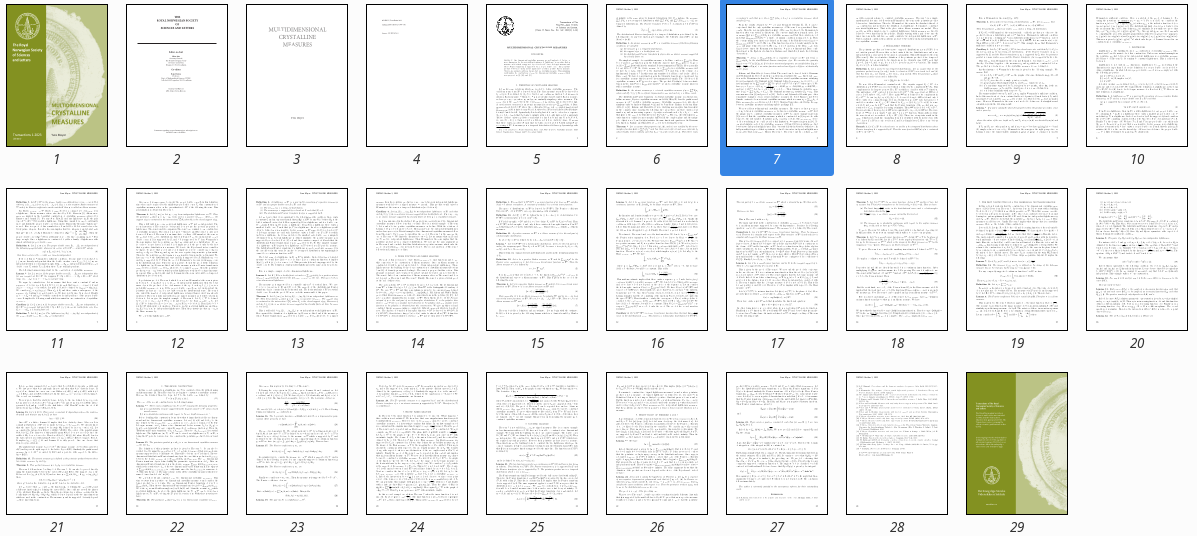
\includegraphics[width=\linewidth]{f/meyershot.png}


\end{frame}

\begin{frame}
	\frametitle{Pavages de Penrose}

	{\bf 1974}. Roger~Penrose,\\
	\emph{
	The role of aesthetics in pure and applied mathematical research
}

\vfill

	\begin{tabular}{ccc}
		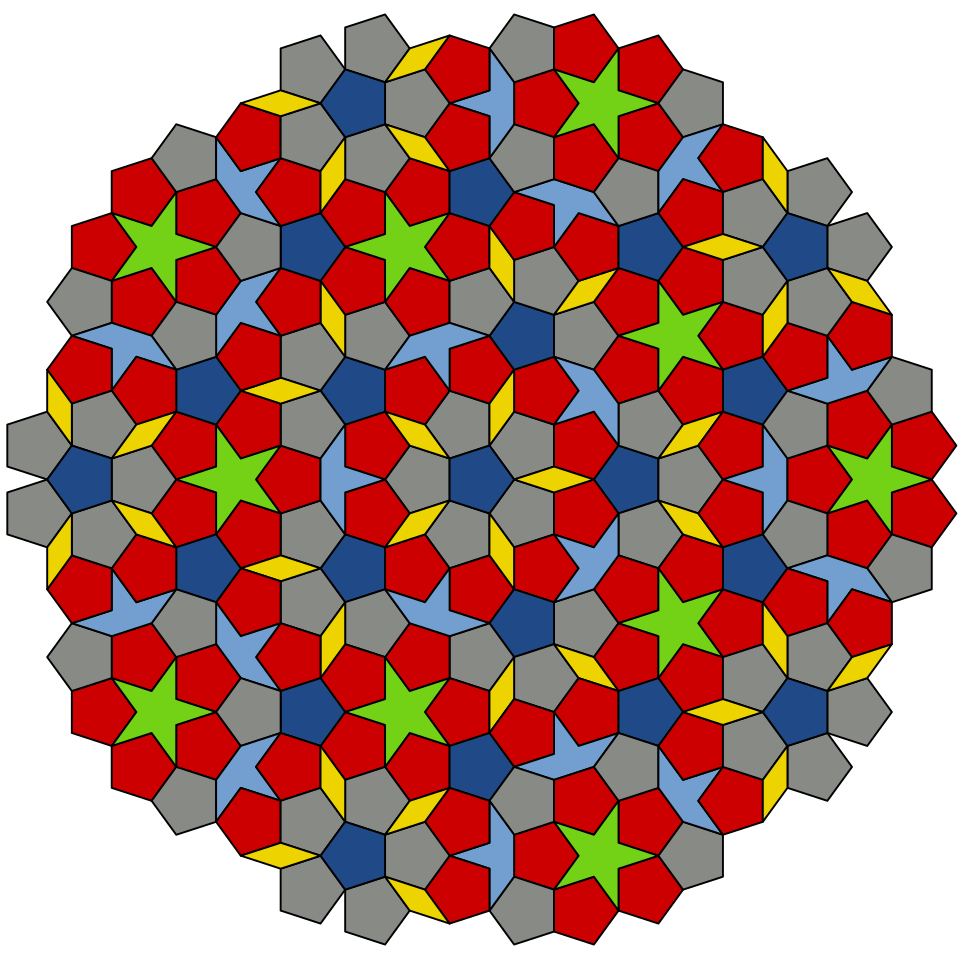
\includegraphics[width=0.25\linewidth]{f/pensrosep1.png}&
		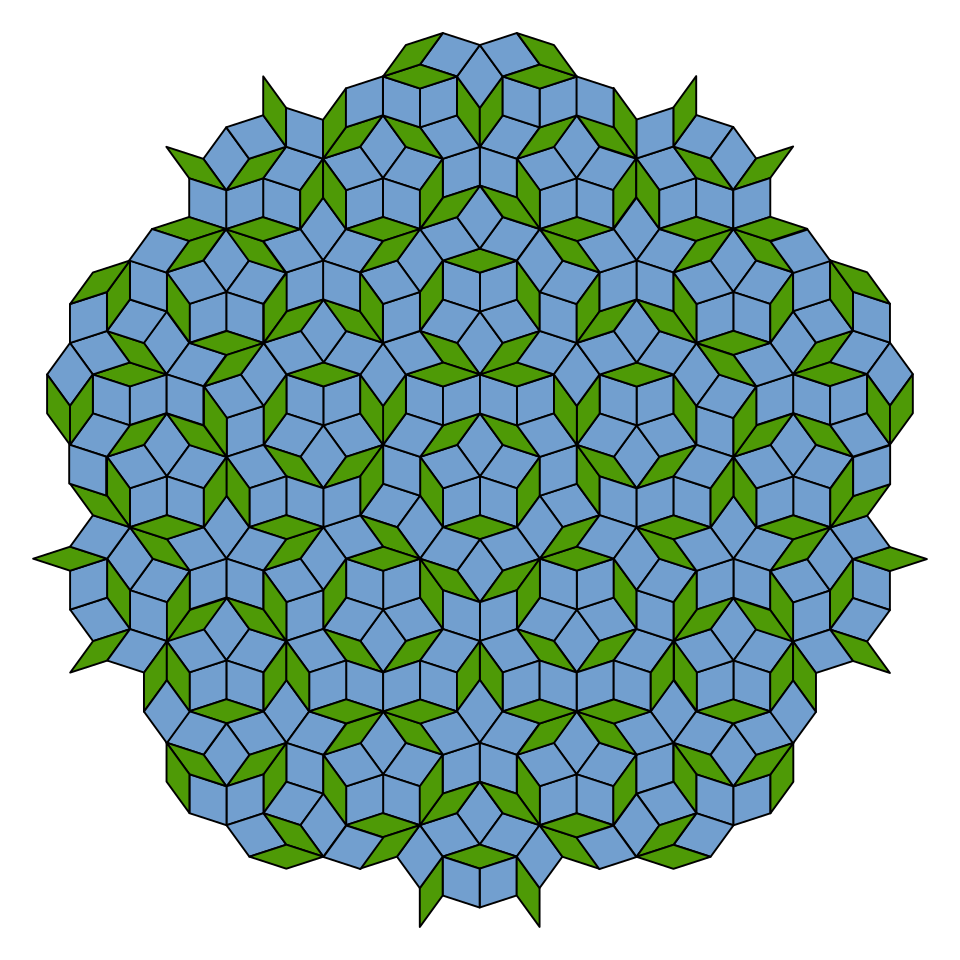
\includegraphics[width=0.3\linewidth]{f/penrombi.png}&
		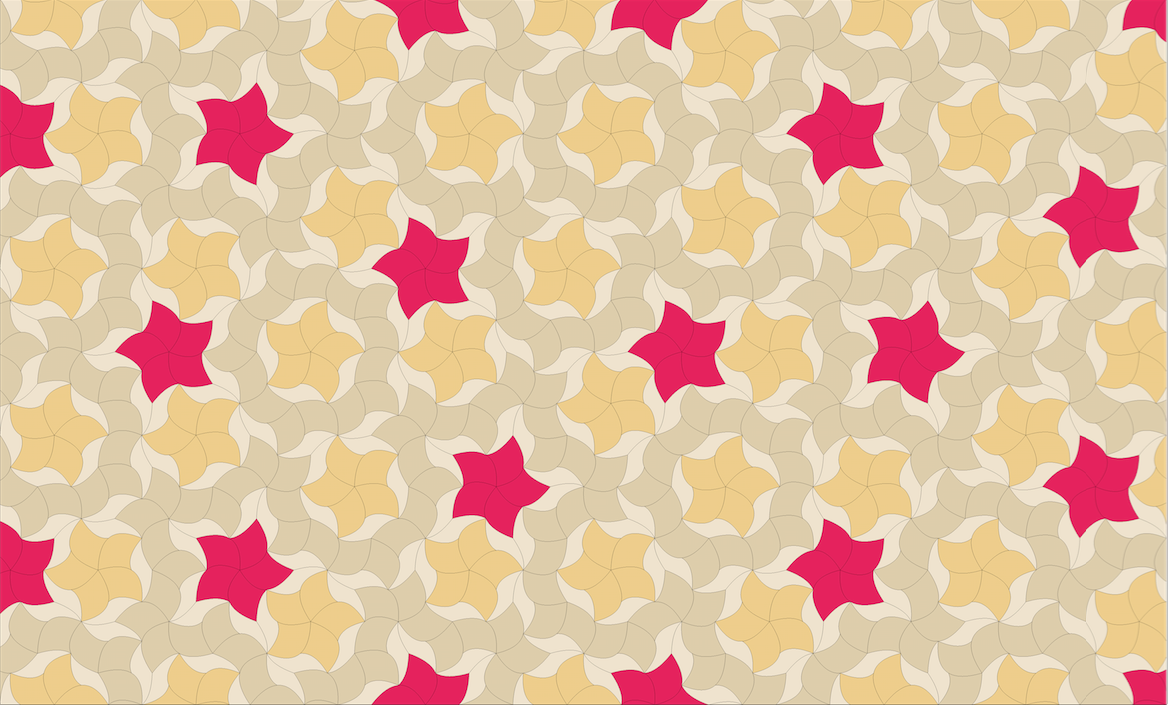
\includegraphics[width=0.35\linewidth]{f/penrosep3.png}\\
		type P1 & type P2 & type P3
	\end{tabular}

\vfill

\end{frame}

\begin{frame}
	\frametitle{Construction mathématique : \underline{cut and project}}

\begin{tabular}{ccc}
	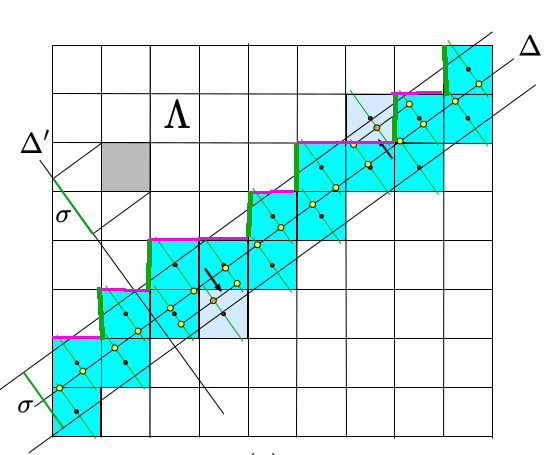
\includegraphics[width=0.3\linewidth]{f/pixels2.png}&
	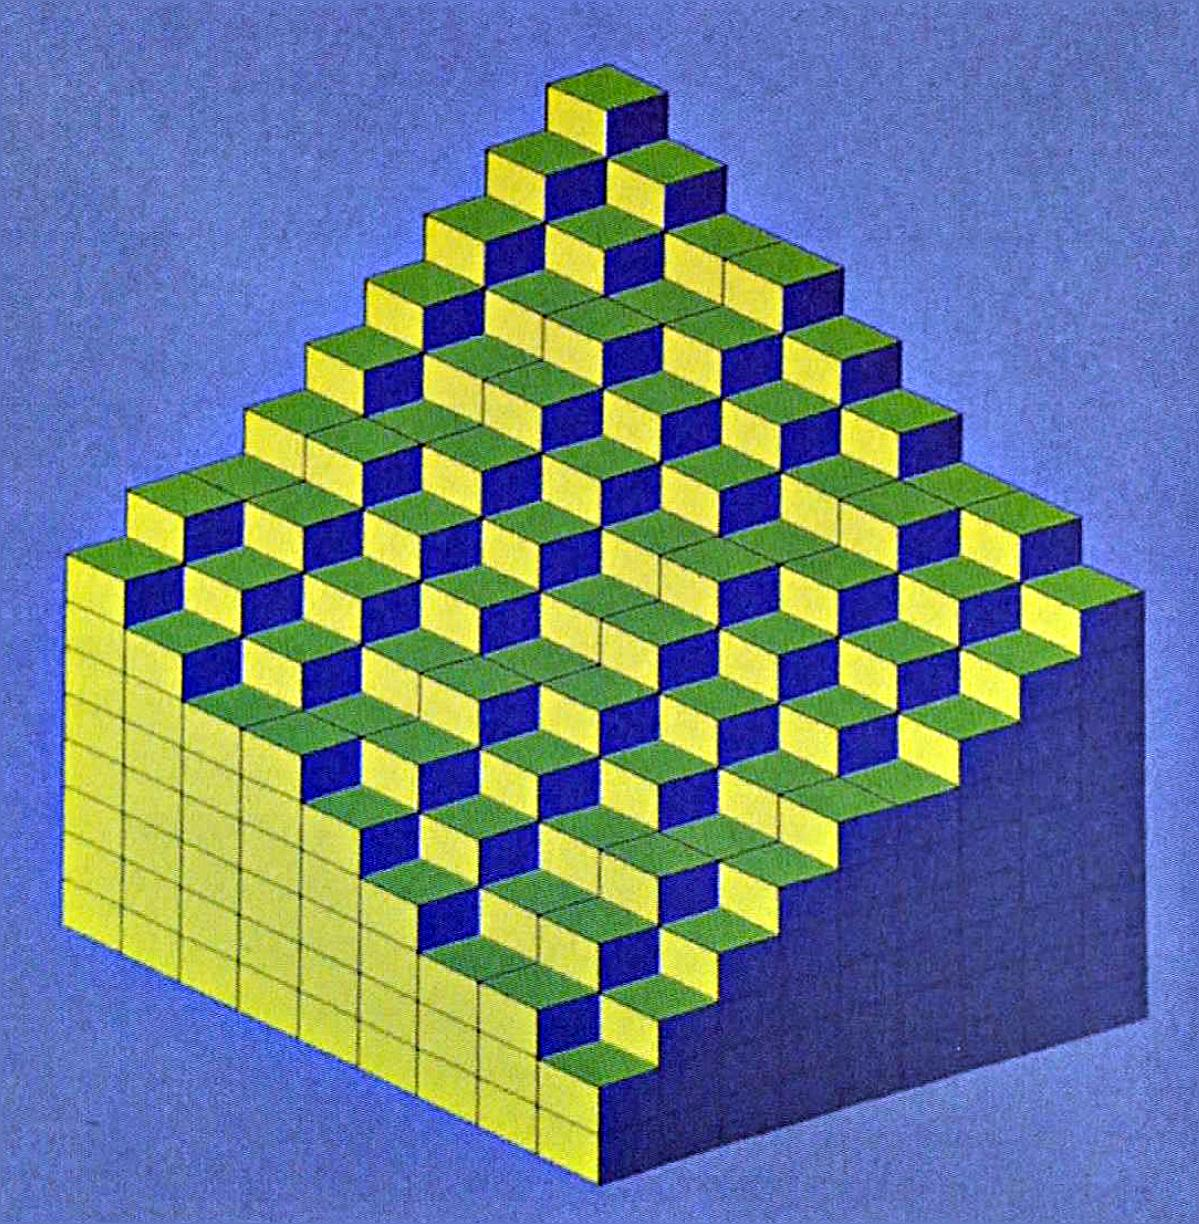
\includegraphics[width=0.28\linewidth]{f/qpt.jpg}&
	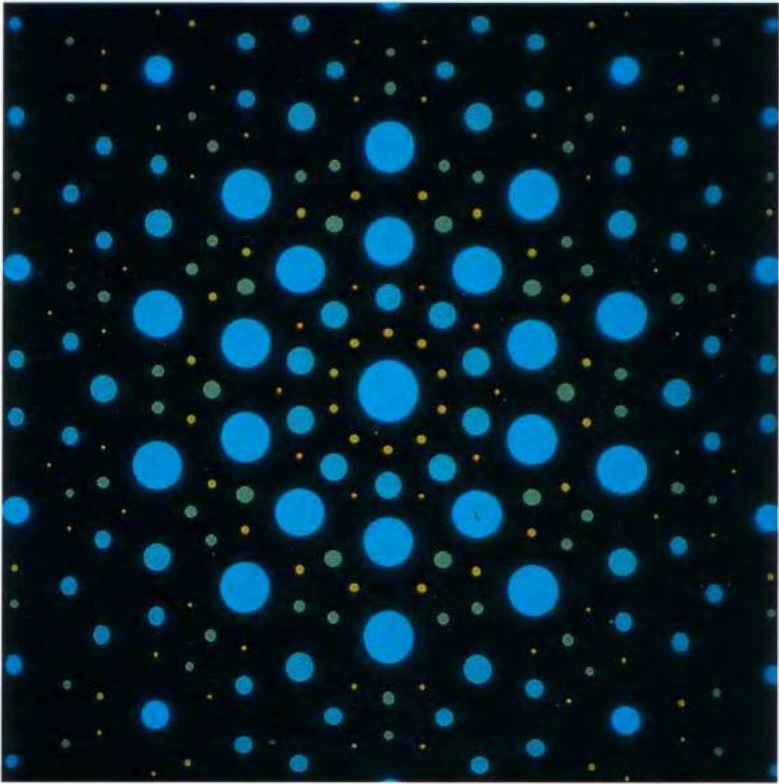
\includegraphics[width=0.26\linewidth]{f/arnofive.png}\\
	quasi-périodicité 1D &
	quasi-périodicité 2D &
	projection~$\Z^5\to\R^2$ \\
	%diffraction du~$\mathrm{Al}_6\mathrm{Mn}$ \\
\end{tabular}
\vfill
\pause
\begin{columns}
	\begin{column}{0.3\linewidth}
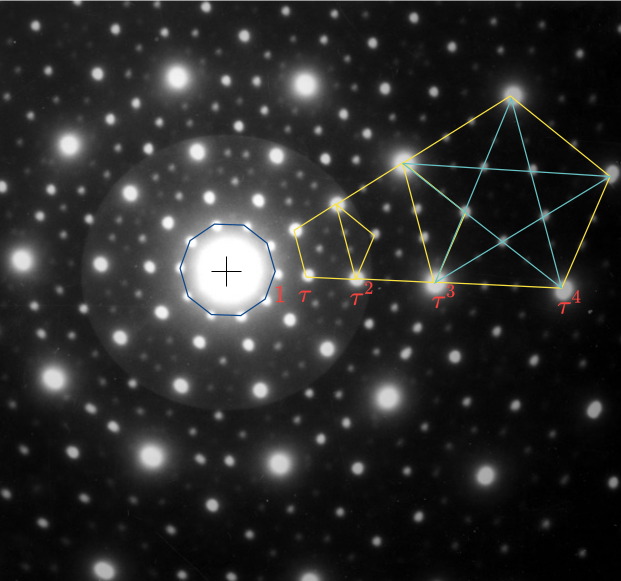
\includegraphics[width=\linewidth]{f/penta.png}\\
\end{column}
	\begin{column}{0.7\linewidth}
diffraction du~$\mathrm{Al}_6\mathrm{Mn}$\\
{\bf 1982} Dan Shechtman {\color{gray}Nobel chimie 2011}
\end{column}
\end{columns}


\end{frame}


\begin{frame}
	\frametitle{Déroulement du stage}

	1. Étudier les travaux de Meyer: {\color{gray}ensembles harmonieux, mesures
	cristallines, pavages apériodiques, quasi-cristaux, $\ldots$}

	2. Illustrer les objets qu'ils décrivent {\color{gray}(pavages avec symétrie d'ordre 13?, remplir l'espace avec tridecahèdres?)}
	\pause

	3. Imprimer les quasicristaux en 3D

	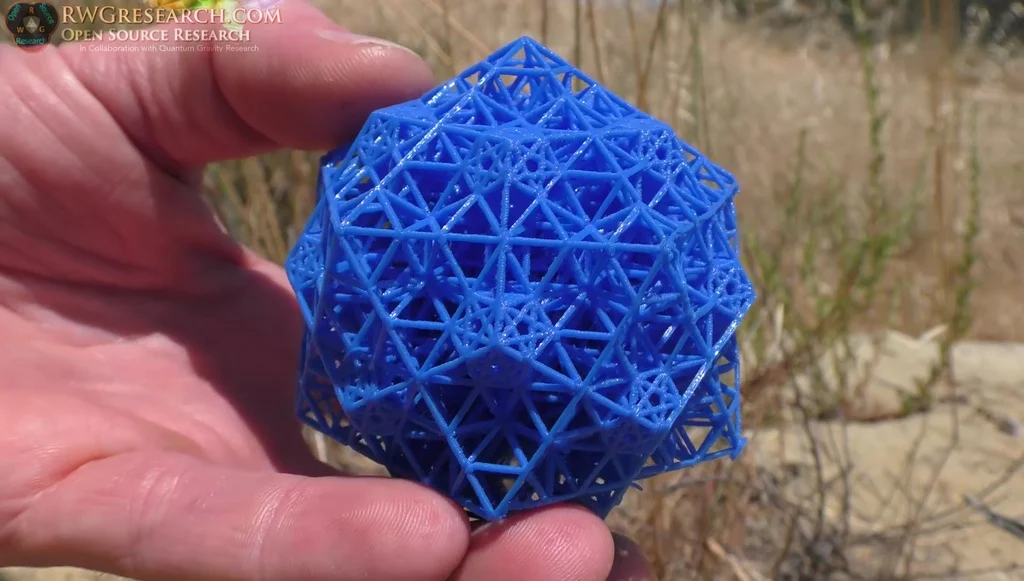
\includegraphics[width=0.43\linewidth]{f/icosablue.png}
	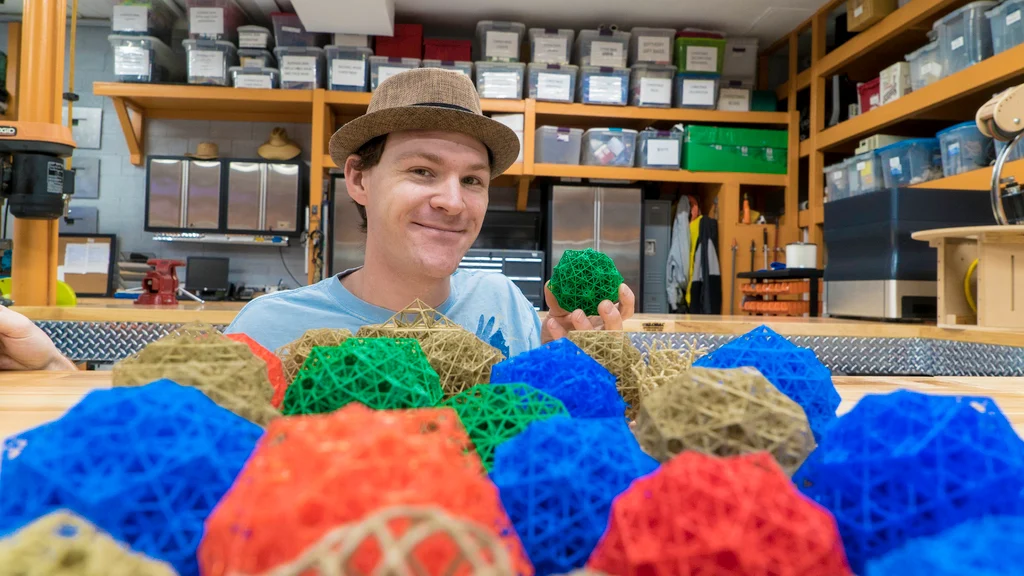
\includegraphics[width=0.43\linewidth]{f/icosamany.png}
	%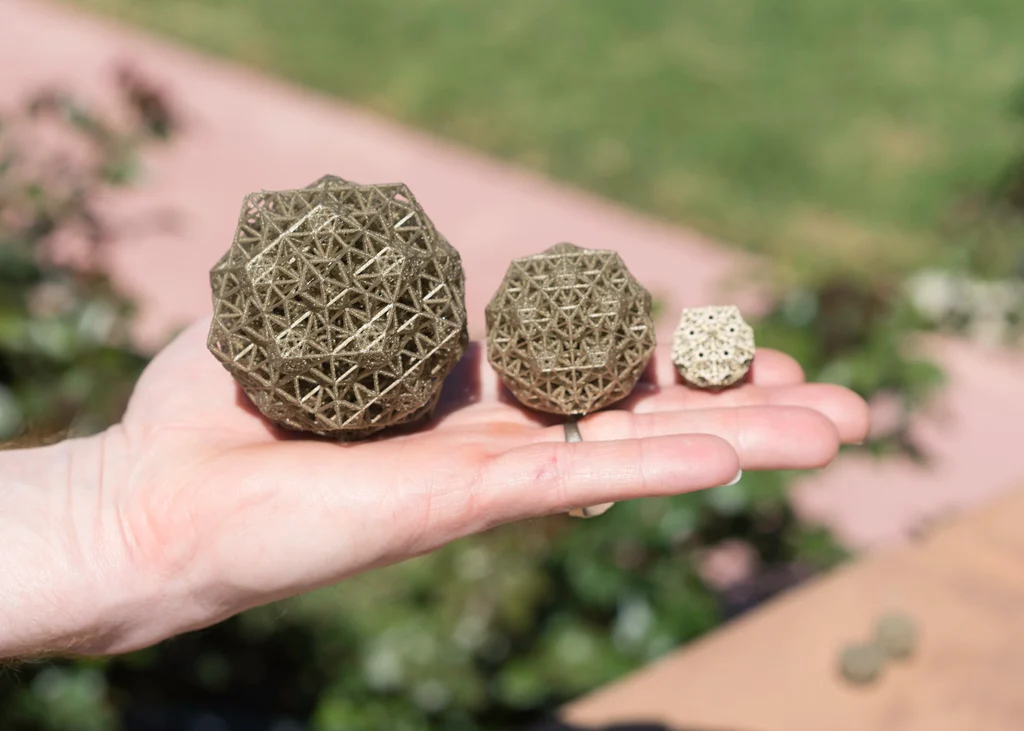
\includegraphics[width=0.3\linewidth]{f/icosaprint.png}
\end{frame}


\end{document}


\addtocounter{framenumber}{-1}


\begin{frame}
ANALOGIES MÉCANIQUE/GÉOMÉTRIE\\
=============================

	\includegraphics[width=0.35\linewidth]{f/sheit2.png}~$ $%
	\includegraphics[height=0.35\linewidth]{f/sheit1.jpg}

	\includegraphics[width=0.7\linewidth]{f/analogy.jpg}

\end{frame}


\begin{frame}
LE PRINCIPE DE MOINDRE ACTION\\
=============================

\vfill

	\begin{columns}
		\begin{column}{0.35\textwidth}
			{\scriptsize Maupertuis 1744\\}
			\includegraphics[width=\linewidth]{f/mauporig.jpg}
		\end{column}
		\begin{column}{0.6\textwidth}
			\pause\footnotesize
			{\bf Proposition} Dans un système mécanique
			$\color{red}\ddot q=-\nabla V(q)$ les trajectoires sont
			minimiseurs d'une action $\color{blue}A[q] =\int S(q(t),\dot q(t))\,\mathrm{d}t$\\\pause{\color{gray}(à reparamétrisation près)}

			\bigskip
			\pause
			{\bf Métrique de Jacobi}
			$S=\sqrt{2(E-V(q))}$

			\bigskip
			\pause
			\begin{tcolorbox}
				{\bf En langage moderne:}\\
				$q =$ courbes géodésiques d'une {\color{blue}variété Riemannienne}
			\end{tcolorbox}
		\end{column}
	\end{columns}


\end{frame}




\begin{frame}
TRAJECTOIRES MÉCANIQUES VS. GÉODÉSIQUES\\
=======================================

\footnotesize
\vfill

\begin{columns}
	\begin{column}{0.45\textwidth}
		Géodésiques sur une variété

		\[\color{blue}
		\mathrm{
			\begin{cases}
		\ddot q^k = -\Gamma^k_{ij}\,\dot q^i\dot q^j\\
				q(0) = p_0\\
				\dot q(0) = v_0
			\end{cases}
	}
		\]

		\includegraphics[width=0.8\linewidth]{f/geocyl2.png}
	\end{column}
	\begin{column}{0.55\textwidth}
		Trajectoires d'un système mécanique

		\[\color{red}\mathrm{
			\begin{cases}
			\ddot q = -\nabla V(q)\\
				q(0) = p_0\\
				\dot q(0) = v_0
			\end{cases}
		}
		\]

		\includegraphics[width=0.8\linewidth]{f/keplers.jpg}
	\end{column}
\end{columns}

\end{frame}




\begin{frame}
THÉORÈME DE PLONGEMENT DE NASH\\
==============================


	{\bf Théorème (Nash 1956).}
	Toute variété riemannienne peut être plongée de manière isométrique dans un
	espace euclidien {\color{gray}de dimension supérieure}.

	\vfill

	\begin{tabular}{cc}
		\includegraphics[width=0.5\linewidth]{f/tissots.jpg} &
		\includegraphics[width=0.45\linewidth]{f/sphere.jpg} \\
		métrique en~$\mathbf{R}^2$ &
		sous-variété de~$\mathbf{R}^3$
	\end{tabular}

\end{frame}


\begin{frame}
SURFACES DE JACOBI-MAUPERTUIS\\
=============================

\end{frame}





\end{document}

%\begingroup
%\setbeamertemplate{background}{\color{twback}\rule{\paperwidth}{\paperheight}}
%\begin{frame}
%HISTOIRE: EX UNGUE LEONEM\\
%=========================
%
%\btweet{f/avatar_newton.jpg}{@hongiiv}{HongChangBum(a)}{iphone 37.6789876}{@yokofakun Your lab notebook is very useful for me. I'm finding variation using Roche454, GATK from Korean population. Thank you :-)}{Thu Sep 16 18:51:39 +0000\,2010}
%
%\end{frame}
%\endgroup

%\begin{frame}
%HISTOIRE: EX UNGUE LEONEM\\
%=========================
%\footnotesize
%
%(in tweets)
%
%Bernoulli, 28/1/1696\\
%guys, new challenge just dropped: find the shape of the ramp where a ball
%slides in least time.  Took me a while to figure it out!
%
%Anonymous Brittanicus, 29/1/1969\\
%(newton solution screenshot)
%
%Bernouilli, 30/1/1969\\
%dammit Newton!
%
%Sir Isaac, 30/1/1969\\
%fml, on et peu et on se connaît trop
%
%L'Hopital, 03/1/1969\\
%lol
%
%Leibniz, 03/1/1969\\
%typical Newton
%
%\end{frame}

\begingroup
\setbeamertemplate{background}{\color{twback}\rule{\paperwidth}{\paperheight}}
\begin{frame}
\tiny
\fontfamily{phv}\selectfont

\colorbox{white}{
	\setlength{\tabcolsep}{.3em}
	\begin{tabular}{cp{0.9\textwidth}}
		\includegraphics[width=0.07\textwidth,align=t]{f/gavatar_bernoulli.png} &
		{\bfseries Jh. Bernoulli}
		\circledmark\ %
		{\color{gray}@Jean67 \hfill 28 Janvier 1696}\newline
		Find the shape of the ramp where a ball
		slides in least time  %Took me a while to figure it out!  \newline
		{\color{blue}\#brachistochrone}
	\end{tabular}
}
%
\pause
\colorbox{white}{
	\setlength{\tabcolsep}{.3em}
	\begin{tabular}{cp{0.9\textwidth}}
		\includegraphics[width=0.07\textwidth,align=t]{f/gavatar_newton.png} &
		{\bfseries Is. Newton}
		\circledmark\ %
		{\color{gray}@sirisaac \hfill 28 Juillet 1696}\newline
		Marre de ces étrangers prétentieux et de leurs questions nulles
	\end{tabular}
}
%
\pause
\colorbox{white}{
	\setlength{\tabcolsep}{.3em}
	\begin{tabular}{cp{0.9\textwidth}}
		\includegraphics[width=0.07\textwidth,align=t]{f/gavatar_barry.png} &
		{\bfseries Anonymous Britannicus}
		\ %\circledmark\ %
		{\color{gray}@barry \hfill 28 Juillet 1696}\newline
		\includegraphics[width=.4\linewidth,align=t]{f/newton.jpg}
	\end{tabular}
}
%
\pause
\colorbox{white}{
	\setlength{\tabcolsep}{.3em}
	\begin{tabular}{cp{0.9\textwidth}}
		\includegraphics[width=0.07\textwidth,align=t]{f/gavatar_bernoulli.png} &
		{\bfseries Jh. Bernoulli}
		\circledmark\ %
		{\color{gray}@Jean67 \hfill 29 Juillet 1696}\newline
		Hahaha {\color{blue}@sirisaac}, I knew you wouldn't resist!\newline
		{\itshape $\ldots$ ex ungue lionem}
	\end{tabular}
}
%
\pause
\colorbox{white}{
	\setlength{\tabcolsep}{.3em}
	\begin{tabular}{cp{0.9\textwidth}}
		\includegraphics[width=0.07\textwidth,align=t]{f/gavatar_leibniz.png} &
		{\bfseries G.W. Leibniz}
		\circledmark\ %
		{\color{gray}@leibnitius \hfill 29 Juillet 1696}\newline
		LOL {\color{blue}@sirisaac @Jean67}
	\end{tabular}
}
%
%\pause
\colorbox{white}{
	\setlength{\tabcolsep}{.3em}
	\begin{tabular}{cp{0.9\textwidth}}
		\includegraphics[width=0.07\textwidth,align=t]{f/gavatar_lhopital.png} &
		{\bfseries L'Hôpital}
		\circledmark\ %
		{\color{gray}@marquisHosp \hfill 29 Juillet 1696}\newline
		Typical Newton
	\end{tabular}
}
%
%\pause
\colorbox{white}{
	\setlength{\tabcolsep}{.3em}
	\begin{tabular}{cp{0.9\textwidth}}
		\includegraphics[width=0.07\textwidth,align=t]{f/gavatar_newton.png} &
		{\bfseries Is. Newton}
		\circledmark\ %
		{\color{gray}@sirisaac \hfill 30 Juillet 1696}\newline
		Le problème est qu'on est peu nombreux et on se connait trop
	\end{tabular}
}
\end{frame}
\endgroup


\begin{frame}
LOI DE SNELL-DESCARTES\\
======================

\only<1>{\includegraphics[width=\linewidth]{f/platja.jpg}}%
\only<2>{\includegraphics[width=\linewidth]{f/platja2.jpg}%
\hspace{-24em}\includegraphics[width=0.13\linewidth]{f/david.jpg}
\hspace{11.5em}\raisebox{12.5em}{\includegraphics[width=0.13\linewidth]{f/tenric2.png}}
	}%
\only<3>{\includegraphics[width=\linewidth]{f/platja3.jpg}%
\hspace{-24em}\includegraphics[width=0.13\linewidth]{f/david.jpg}
\hspace{11.5em}\raisebox{12.5em}{\includegraphics[width=0.13\linewidth]{f/tenric2.png}}
	}%
\only<4>{\includegraphics[width=\linewidth]{f/platja4.jpg}%
\hspace{-24em}\includegraphics[width=0.13\linewidth]{f/david.jpg}
\hspace{11.5em}\raisebox{12.5em}{\includegraphics[width=0.13\linewidth]{f/tenric2.png}}
	}%
\only<5>{\includegraphics[width=\linewidth]{f/platja4.jpg}%
\hspace{-24em}\includegraphics[width=0.13\linewidth]{f/david.jpg}
\hspace{11.5em}\raisebox{12.5em}{\includegraphics[width=0.13\linewidth]{f/tenric2.png}}%
	\hspace{-5em}\raisebox{3em}{\includegraphics[width=0.25\linewidth]{f/msnellonly.png}}
	}%

\end{frame}


%\begin{frame}
%LOI DE SNELL-DESCARTES ITÉRÉE\\
%=============================
%
%\only<1>{\includegraphics[width=\linewidth]{f/platjaroad.jpg}}%
%\only<2>{\includegraphics[width=\linewidth]{f/platjaroad2.png}}%
%\only<3>{\includegraphics[width=\linewidth]{f/platjaroad3.png}%
%\hspace{-15em}\raisebox{4em}{\includegraphics[width=0.45\linewidth]{f/snell3K.png}}%
%	}%
%
%\end{frame}

\begin{frame}
LOI DE SNELL-DESCARTES ITÉRÉE\\
=============================


\setlength{\fboxsep}{0pt}
\begin{tabular}{lp{0.5\textwidth}}
\fbox{\includegraphics[align=t,width=0.34\linewidth]{f/snell6.png}} &
	\LARGE
	\color{blue}$\displaystyle\frac{\sin\theta_i}{v_i}=K$
	\\
	\pause
\fbox{\includegraphics[align=t,width=0.34\linewidth]{f/snell46.png}} &
	\color{blue}
	\Large
	$\frac{\sin\theta(x)}{v(x)}=K$\newline
	$ $\newline
	$\frac{\sin\arctan\frac{dy}{dx}}{v(x)}=K$\newline
	$ $\newline
	$\frac{y'(x)}{v(x)\sqrt{1+y'(x)^2}}=K$
\end{tabular}


\end{frame}



\begin{frame}
OPTIQUE VS. MÉCANIQUE\\% : EXEMPLES\\
=====================%===========

\tiny
\begin{tabular}{lll}
	\includegraphics[width=0.3\linewidth]{f/wolframcyc.png}&
	\includegraphics[width=0.3\linewidth]{f/wikipoincare.png}&
	\includegraphics[width=0.3\linewidth]{f/wikiparabo.png}\\
	Brachistochrone~: $\color{blue} v(y)=1/\sqrt{y}$ &
	demi-plan de Poincaré~: $\color{blue} v(y)=1/y$ &
	tir parabolique~: $\color{blue} v(y)=y/\sqrt{1+y^2}$\\
	& & \\
	& & \\
	& & \\
\end{tabular}

\vfill

\begin{tabular}{ccc}
	\includegraphics[width=0.25\linewidth]{f/snellcirc.png}&
	\includegraphics[width=0.2\linewidth]{f/twomercators.png}%
	\includegraphics[width=0.2\linewidth]{f/twohammers2.jpg}&
	\includegraphics[width=0.3\linewidth]{f/geodesicsn.png}\\
	gravitation~: $\color{blue}v(r)=\textbf{?}$ &
	grands cercles~: $\color{blue}v(x,y)=\textbf{?}$ &
	géodésiques~: $\color{blue}v=\left(\begin{smallmatrix}E&F\\F&G\end{smallmatrix}\right)^{-1}$ \\
		& & \\
		& & $\color{red}\ddot x^k = \Gamma^k_{ij}\dot x^i\dot x^j$
\end{tabular}

\end{frame}


\begin{frame}\scriptsize
\setlength{\parskip}{.8em}
$ $

	{\bf DÉROULEMENT DU STAGE}

1. Généraliser la loi de Snell-Descartes~:

	\begin{tabular}{cc}
		\includegraphics[width=0.18\linewidth]{f/snellellipse2.png}&
		\includegraphics[width=0.18\linewidth]{f/snell2d2.png}\\
		\tiny\color{blue}milieux non-isotropes &
		\tiny\color{blue} partitions 2D
	\end{tabular}

	2. Étude théorique de plusieurs exemples
	(plan de Poincaré, orbites, etc).

{\color{gray}
3. En option~: implementation informatique, étude historique
}

\vfill

	{\bf TECHNIQUES À APPRENDRE}

- calcul des variations~:
	$\displaystyle
	\color{red}
	\min\int L(q(t),\dot q(t))\mathrm{d}\,t
	\quad\implies\quad
	\frac{\partial L}{\partial q}
	-\frac{\mathrm{d}}{\mathrm{d}t}\frac{\partial L}{\partial\dot q}=0$

- géométrie Riemannienne~:
		$\displaystyle\color{red}
		L=E\dot x^2+2F\dot x\dot y+G\dot y^2
		\quad\implies\quad
		\ddot q^k = \Gamma^k_{ij}\dot q^i\dot q^j$

- aproximation de solutions d'une EDO~:
	$\displaystyle\color{red}\lim_{h\to 0}q^h(t)=q(t)$

\end{frame}

\appendix

\begin{frame}\small
GÉODÉSIQUES SUR UNE VARIÉTÉ RIEMANNIENNE\\
========================================

Sur chaque point $x\in\R^2$ il y a une
	matrice~$\color{red} g_x=\begin{pmatrix}E&F\\F&G\end{pmatrix}$

		Longueur d'un vecteur~$\left\|v_x\right\|_{\color{red}g_x}:=\sqrt{{\color{red}g_x}(v_x,v_x)}$

%	{\color{blue}(dessin avec indicatrices de Tissot)}

Longueur d'une trajectoire~$\gamma:[a,b]\to\R^2$
	\[
		{\color{red}\ell}(\gamma)
		:=
		\int_a^b\left\|\dot\gamma(t)\right\|_{\color{red}g_{\gamma(t)}}\mathrm{d}t
	\]

EDO satisfaite par les courbes de longueur minimale~:
	\[
		\begin{cases}
			\ddot x
			= {\color{red}\Gamma_1^{11}}\dot x^2
			+ {\color{red}\Gamma_1^{12}}\dot x\dot y
			+ {\color{red}\Gamma_1^{22}}\dot y^2\\
			\ddot y
			= {\color{red}\Gamma_2^{11}}\dot x^2
			+ {\color{red}\Gamma_2^{12}}\dot x\dot y
			+ {\color{red}\Gamma_2^{22}}\dot y^2\\
		\end{cases}
	\]

	\vfill

	$\color{red}\Gamma^k_{ij} = $ fonctions de~$\color{red}E,F,G$ et leurs
	dérivées
\end{frame}



%%\tweet{f/gavatar_bernoulli.png}{Jh. Bernoulli\ \circledmark\ }{28 Jan 1696}{
%\tweet{f/gavatar_bernoulli.png}{Jh. Bernoulli}{28 Jan 1696}{%
%	Find the shape of the ramp where a ball%
%	slides in least time.  Took me a while to figure it out!%
%}



\end{document}


% vim:sw=2 ts=2 spell spelllang=fr:
